\documentclass[border=5pt]{standalone}
\usepackage{tikz,graphicx,amsmath,amssymb,xcolor}\usepackage{fontspec,xeCJK}\setmainfont{Helvetica}\setCJKmainfont{PingFang SC}
\usetikzlibrary{arrows.meta}
\definecolor{ink}{HTML}{203D46}\definecolor{teal}{HTML}{277A80}\definecolor{pale}{HTML}{EFF6F5}\definecolor{warm}{HTML}{F6ECDD}
\begin{document}\begin{tikzpicture}[x=1mm,y=1mm,font=\fontsize{11}{14}\selectfont,text=ink]
\path[use as bounding box] (0,0) rectangle (105,260);
\node[anchor=north west,font=\bfseries\fontsize{16}{19}\selectfont] at (3,258) {MAE：一张图走完整条链};
\node[anchor=north west,text width=98mm,font=\fontsize{10}{13}\selectfont] at (3,248) {训练：$A\to B\to C$，D 对遮挡像素监督 B/C。使用：完整图走 $B\to E$。尺寸以 ViT-L/16 为例，CLS 单列计数。};
\fill[pale,rounded corners=2mm] (1,191) rectangle (104,232);
\node[anchor=north west,text=teal,font=\bfseries\fontsize{12}{15}\selectfont] at (4,230) {A 随机藏块 · §3};
\node[anchor=north west,text width=66mm,inner sep=0] at (4,222) {$224\times224\times3\rightarrow196$ 块\\随机藏 $75\%$：147 块\\49 可见块保留原位置\\遮挡集 $M$ 只用于训练目标};
\node[anchor=center,inner sep=0] at (88,208) {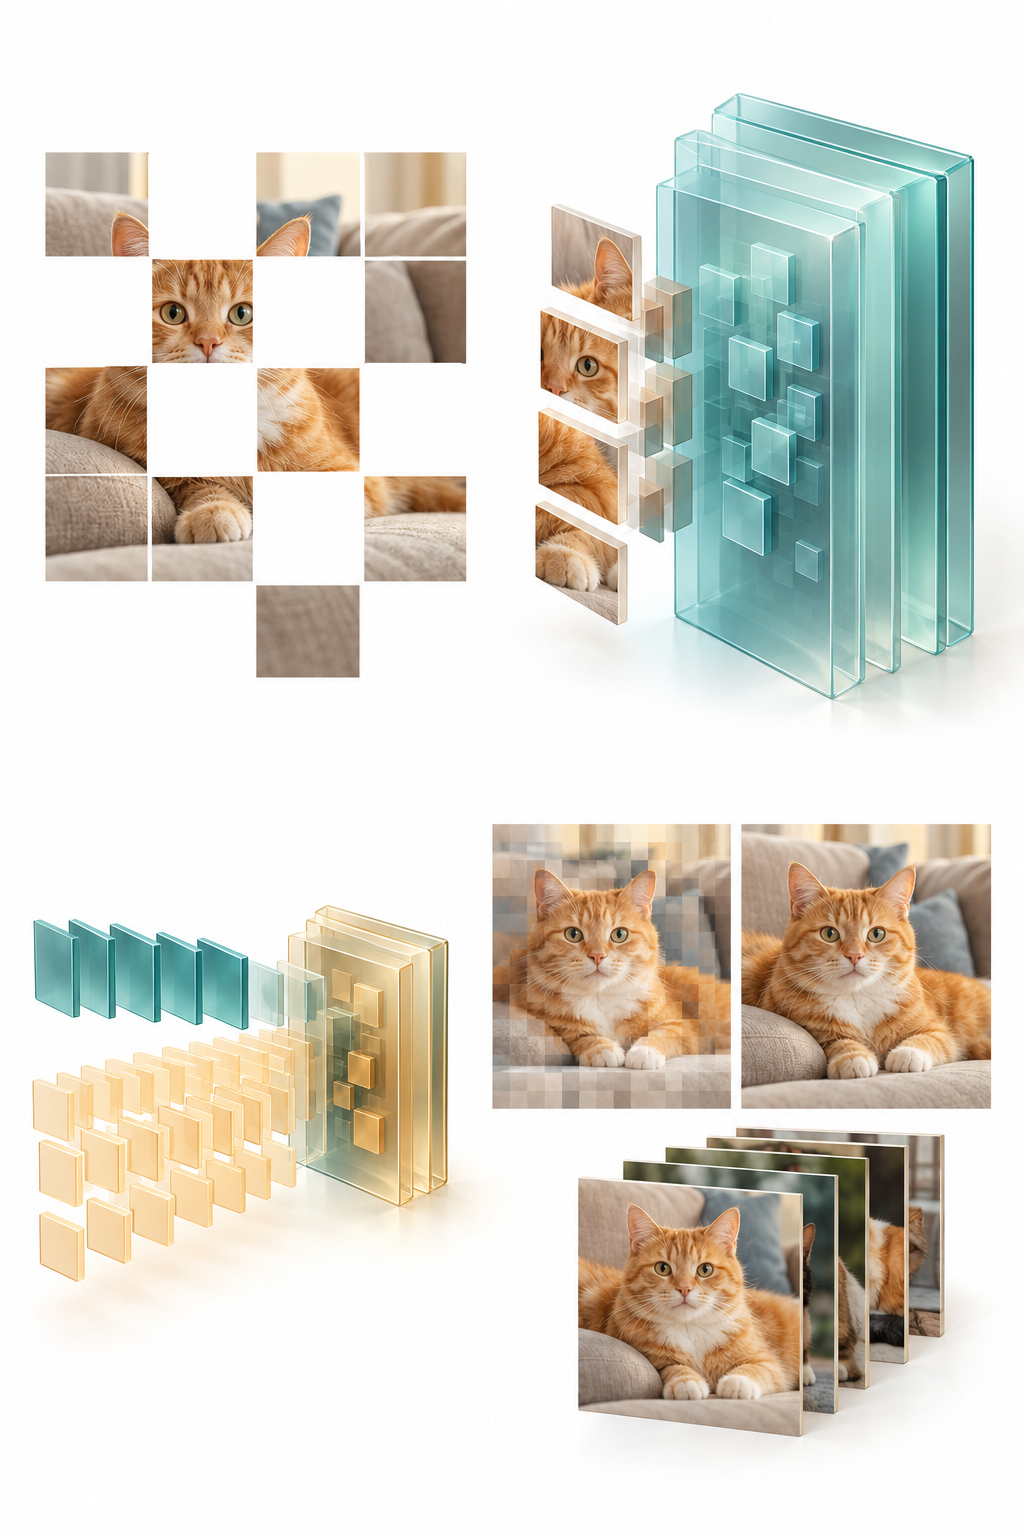
\includegraphics[width=26mm,height=31mm,keepaspectratio,viewport=25 886 510 1456,clip]{mae-imagegen-draft.png}};
\draw[-{Latex[length=2mm]},teal,line width=.7pt] (52.5,190.5) -- (52.5,187);
\fill[pale,rounded corners=2mm] (1,145) rectangle (104,186);
\node[anchor=north west,text=teal,font=\bfseries\fontsize{12}{15}\selectfont] at (4,184) {B 重编码器 · §3};
\node[anchor=north west,text width=66mm,inner sep=0] at (4,176) {只处理可见块 + CLS\\ViT-L：$50\times1024$\\24 层注意力与 MLP\\空白 mask 不进这里};
\node[anchor=center,inner sep=0] at (88,162) {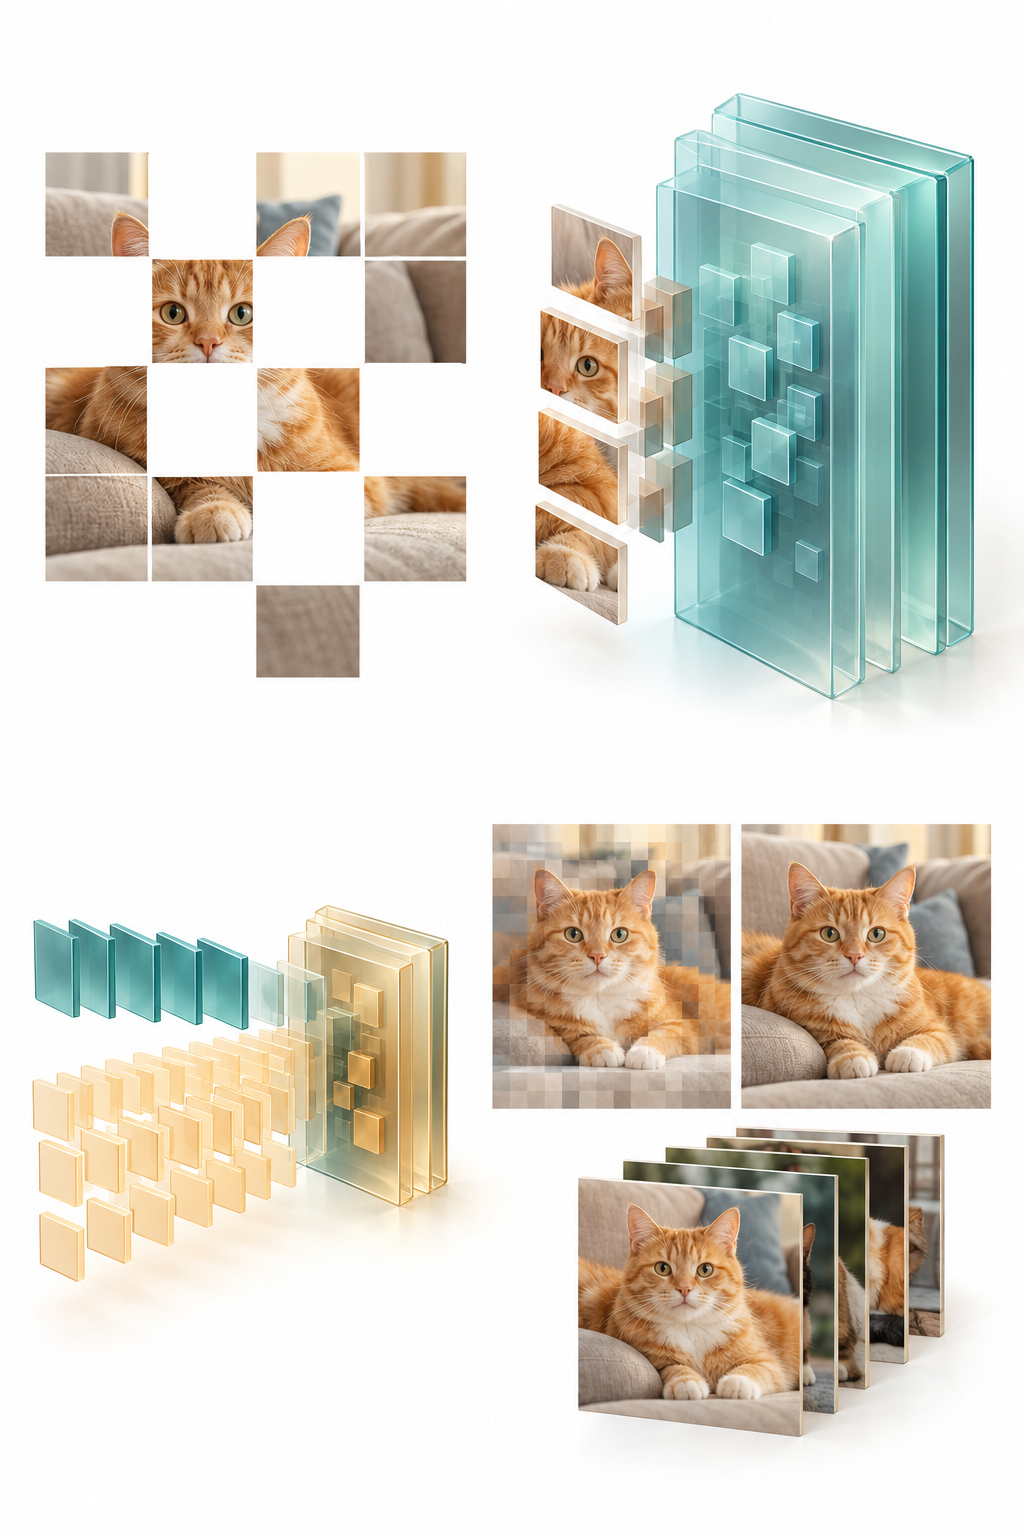
\includegraphics[width=26mm,height=31mm,keepaspectratio,viewport=520 846 1000 1486,clip]{mae-imagegen-draft.png}};
\draw[-{Latex[length=2mm]},teal,line width=.7pt] (52.5,144.5) -- (52.5,141);
\fill[pale,rounded corners=2mm] (1,99) rectangle (104,140);
\node[anchor=north west,text=teal,font=\bfseries\fontsize{12}{15}\selectfont] at (4,138) {C 轻解码器 · §3};
\node[anchor=north west,text width=66mm,inner sep=0] at (4,130) {投影到 512 维，补回 mask\\恢复顺序 + 解码位置\\8 层输出完整图块预测\\$196\times768$ 像素值};
\node[anchor=center,inner sep=0] at (88,116) {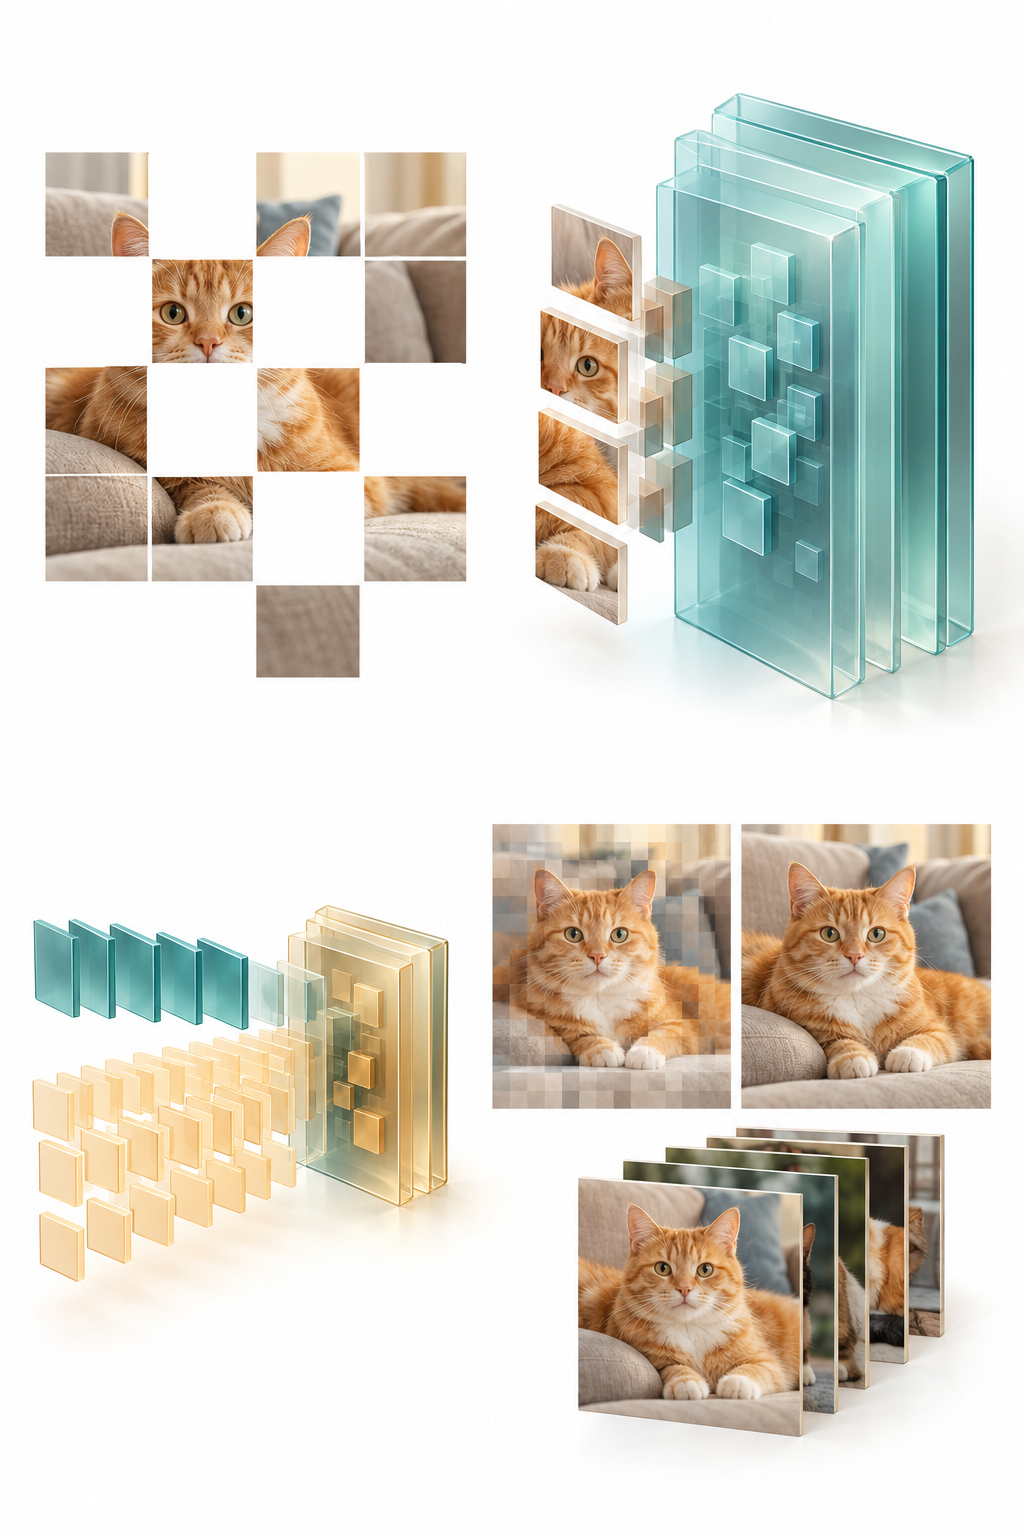
\includegraphics[width=26mm,height=31mm,keepaspectratio,viewport=20 66 520 801,clip]{mae-imagegen-draft.png}};
\draw[-{Latex[length=2mm]},teal,line width=.7pt] (52.5,98.5) -- (52.5,95);
\fill[warm,rounded corners=2mm] (1,53) rectangle (104,94);
\node[anchor=north west,text=teal,font=\bfseries\fontsize{12}{15}\selectfont] at (4,92) {D 遮住的部分算损失 · §3};
\node[anchor=north west,text width=66mm,inner sep=0] at (4,84) {预测与原图块作像素 MSE\\只在147个遮挡块平均\\可用每块均值/方差归一化\\梯度更新 B 与 C};
\node[anchor=center,inner sep=0] at (88,70) {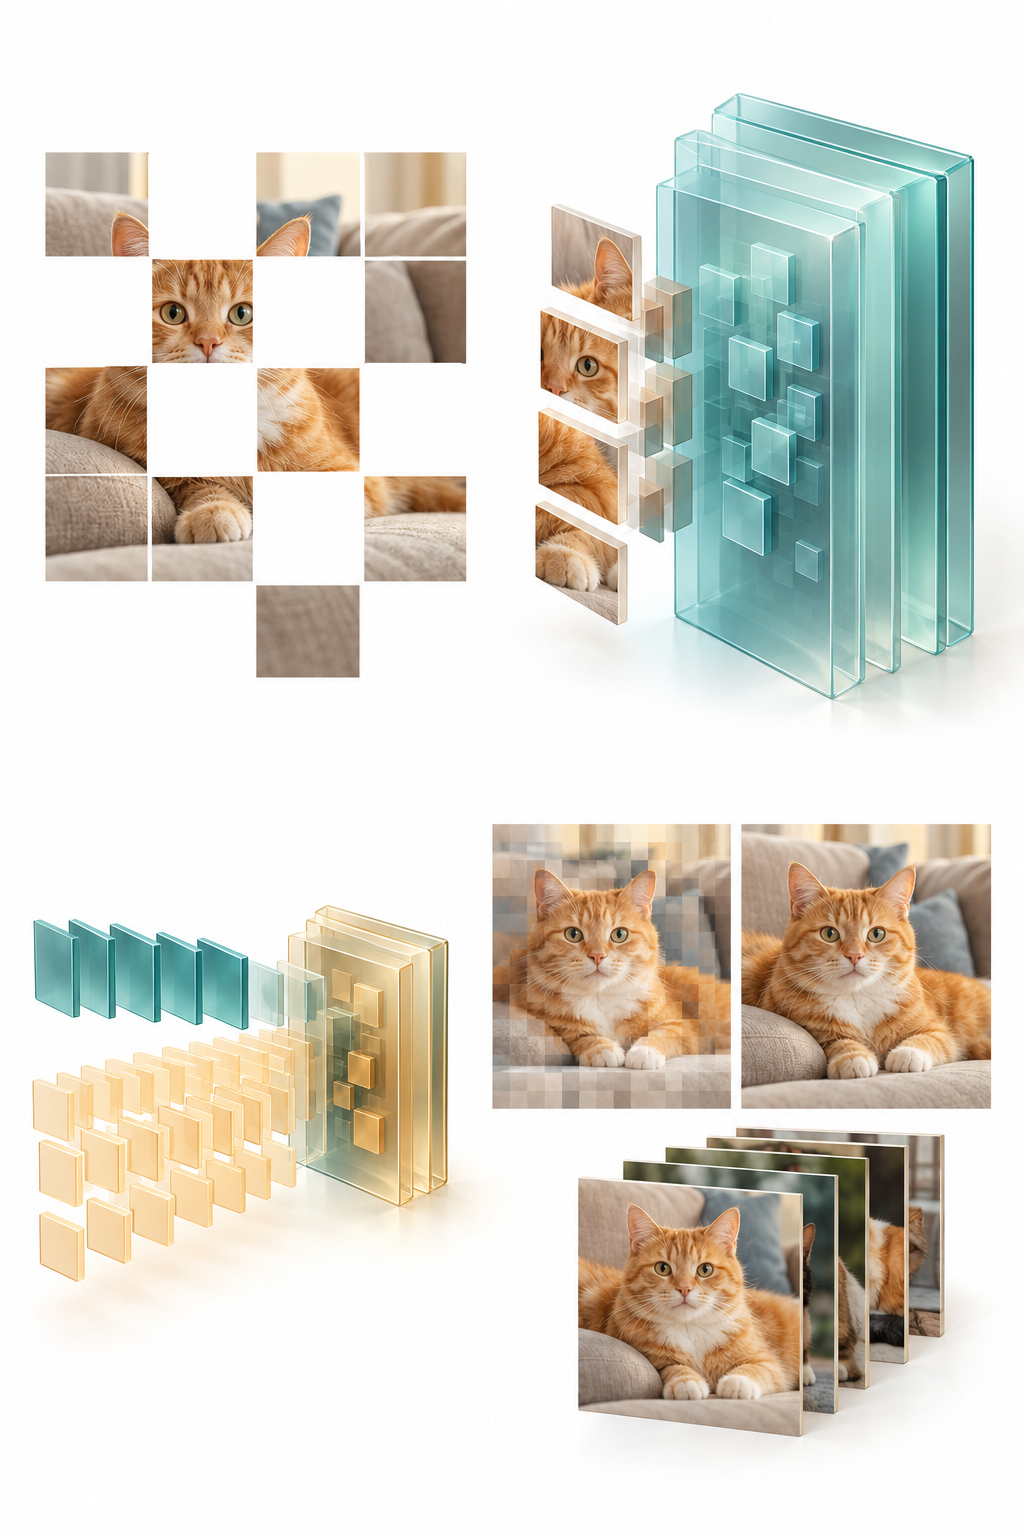
\includegraphics[width=26mm,height=31mm,keepaspectratio,viewport=530 336 1010 826,clip]{mae-imagegen-draft.png}};
\draw[-{Latex[length=2mm]},teal,line width=.7pt] (52.5,52.5) -- (52.5,49);
\fill[pale,rounded corners=2mm] (1,7) rectangle (104,48);
\node[anchor=north west,text=teal,font=\bfseries\fontsize{12}{15}\selectfont] at (4,46) {E 下游拿走编码器 · §4–5};
\node[anchor=north west,text width=66mm,inner sep=0] at (4,38) {丢掉解码器，输入完整图\\分类头微调或冻结读出\\检测/分割加任务网络\\重建只是练习，表示才是成果};
\node[anchor=center,inner sep=0] at (88,24) {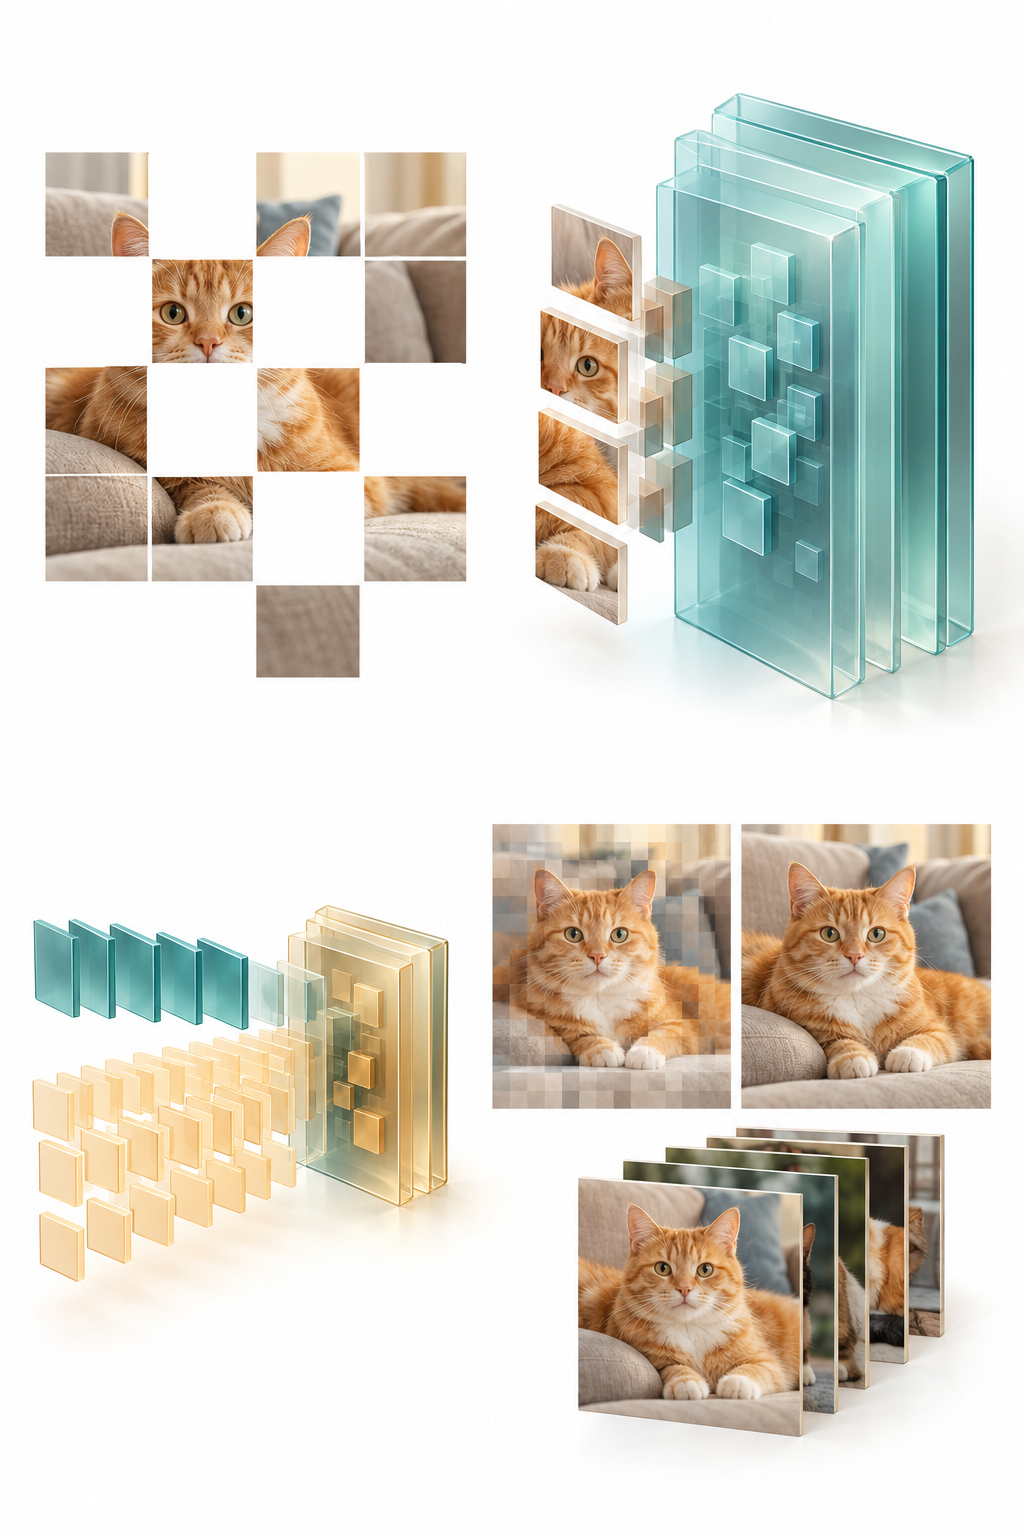
\includegraphics[width=26mm,height=31mm,keepaspectratio,viewport=600 26 1010 376,clip]{mae-imagegen-draft.png}};
\end{tikzpicture}\end{document}